\documentclass{beamer}

\usepackage{bm}
\usepackage{pgfpages}
\usepackage{graphicx}
	\graphicspath{{../images/}} 
%\usepackage{cite}
\usepackage{ragged2e}
\usepackage{parskip}
\usepackage{wrapfig}
\usepackage{array}
\usepackage{float}
\usepackage[english]{babel}
\usepackage{lipsum}
\usepackage{caption}
\usepackage{subcaption}
\usepackage{graphicx}
\usepackage[linesnumbered,ruled]{algorithm2e}
\usepackage{courier}
\usepackage{hyperref}
\hypersetup{colorlinks=true,allcolors=blue}
\usepackage{listings}
\lstset{
    basicstyle=\ttfamily,
    frame=none, 
    breaklines=true,
    numbers=left,
    xleftmargin=2.5em,
    framexleftmargin=0em,
    emphstyle=\textbf,
    float=t
}
\lstdefinestyle{ocl}{
    emph={
        context, inv
    }
}
\lstdefinestyle{cbp}{
    basicstyle=\ttfamily\scriptsize,
    emph={
        session, create, of, type,
        set, to, add, hire
    }
}
\lstdefinestyle{xmi}{
    basicstyle=\ttfamily\scriptsize,
    emph={
        Node, children
    }
}
\lstdefinestyle{xml}{
    basicstyle=\ttfamily\scriptsize,
    emph={
        register, create, add, to, resource,
        from, eattribute, remove, ereference,
        set, unset, session, Roy, Jen,
        Moss, Richmond
    }
}
\lstdefinestyle{java}{
    basicstyle=\ttfamily\scriptsize,
    emph={
        case, $unset$,
        instanceof, else, if, void,
        new, UnsetEAttributeEvent,
        UnsetEReferenceEvent,
        @override, public, class, extends
    }
}
\lstdefinestyle{eol}{
    basicstyle=\ttfamily\scriptsize,
    emph={
        type,
        var, new, for, in, create, set, of, with, 
        unset, to, add, remove, delete, register, move,
        from, position, from, move-within, session, \.
    }
}

\definecolor{UniBlue}{RGB}{73,111,160}
\definecolor{Black}{RGB}{0,0,0}
\definecolor{Gray}{RGB}{240,240,240}
\setbeamercolor{title}{fg=UniBlue}
\setbeamercolor{frametitle}{fg=UniBlue, bg=Gray}
\setbeamercolor{structure}{fg=UniBlue}
\beamertemplatenavigationsymbolsempty
\setbeamertemplate{itemize items}[circle]
\setbeamertemplate{footline}[frame number]
\setbeamertemplate{bibliography item}{\insertbiblabel}
\setbeamertemplate{caption}[numbered]

\lstset{escapeinside={<@}{@>}}

%\setbeameroption{show notes on second screen}


\begin{document}

\title{Towards Efficient Loading of\\Change-Based Models}
%\subtitle{Evidence from India}
\author[Alfa, Yohannis] % (optional, for multiple authors)
{Alfa Yohannis \and Horacio Hoyos Rodriguez$^{*}$ \\ \and Fiona Polack$^{**}$ \and Dimitris Kolovos}
\institute[University of York] % (optional)
{
    Department of Computer Science, University of York, United Kingdom\\$^{**}$School of Computing and Maths, Keele University, United Kingdom\\
    \hfill\\
    \scriptsize \{ary506, dimitris.kolovos\}@york.ac.uk
    \\$^{*}$horacio\_hoyos\_rodriguez@ieee.org
    \\$^{**}$f.a.c.polack@keele.a.cuk\\
    \hfill\\
}

\date[]{\scriptsize
ECMFA 2018\\
Wednesday, 27 June 2018\\
Toulouse, France
}

\titlegraphic{\includegraphics[height=1.5cm]{uoy.pdf}}
\frame{\titlepage}

\begin{frame}[fragile]
\section{Introduction}
\frametitle{Introduction}
\begin{itemize}
    \item Persisting changes made to a large model can be computationally expensive. 
    \item As an alternative approach, change-based persistence (CBP) persist changes of a model instead of persisting its state.
\end{itemize}

\begin{columns}
\begin{column}[t]{0.51\linewidth}
\begin{lstlisting}[style=xmi,caption={The tree model persisted in a state-based format (XMI).},label=lst:xmimodel]
<Node id="n1" name="A">
<children id="n2" name="B"/>
</Node>
\end{lstlisting}
\end{column}
\begin{column}[t]{0.49\linewidth}
\begin{lstlisting}[style=eol,caption={The tree model persisted in a change-based format.},label=lst:cbpmodel]
create n1 type Node
set n1.name to "A"  
create n2 type Node
set n2.name to "B"  
create n3 type Node
set n3.name to "C"  
add n2 to n1.children   
add n3 to n1.children
remove n3 from n1.children   
delete n3
\end{lstlisting}
\end{column}
\end{columns}

%\note{
%\begin{itemize}
%    \item Note
%\end{itemize}
%}
\end{frame}

\begin{frame}
\section{Running Example}
\frametitle{Running Example}
    \begin{figure}[ht]
        \begin{subfigure}[t]{0.45\linewidth}
            \centering
            \includegraphics[width=0.8\linewidth]{node_metamodel}
            \caption{The tree metamodel (EMF/Ecore).}
            \label{fig:tree_metamodel}
        \end{subfigure}
        \hfill
        \begin{subfigure}[t]{0.45\linewidth}
            \centering
            \includegraphics[width=\linewidth]{initial_chart}
            \caption{A tree model that conforms to the  metamodel.  Node \textbf{n3} is created and then deleted. Its CBP is presented in Listing 2.}
            \label{fig:initial_model}
        \end{subfigure}
        \caption{Running example of a metamodel and a conformant model.}
        \label{fig:append_speed}
    \end{figure}
\end{frame}

\begin{frame}
\section{Benefits and Drawbacks}
\frametitle{Benefits and Drawbacks}
\begin{itemize}
    \item Benefits of CBP:
    \begin{itemize}
        \item Faster change-detection, model comparison and merging.
        \item Carries information useful for model analytics.
    \end{itemize} 
    \item Drawbacks of CBP:
    \begin{itemize}
        \item Large, ever-growing CBP files.
        \item \textbf{Increase on model loading time} (need to replay all changes).
    \end{itemize} 
\end{itemize}
\end{frame}

\begin{frame}[fragile]
\section{Loading Time Optimisation}
\frametitle{Loading Time Optimisation}

\begin{columns}
\begin{column}[t]{0.5\linewidth}
\begin{lstlisting}[style=eol,caption={A tree model persisted in change-based.},label=lst:cbpmodel]
create n1 type Node
set n1.name to "A"  
create n2 type Node
set n2.name to "B"  
<@\textcolor{red}{\textbf{create n3 type Node}}@> 
<@\textcolor{red}{\textbf{set n3.name to "C"}}@>   
add n2 to n1.children   
<@\textcolor{red}{\textbf{add n3 to n1.children}}@> 
<@\textcolor{red}{\textbf{remove n3 from n1.children}}@> 
<@\textcolor{red}{\textbf{delete n3}}@> 
\end{lstlisting}        
\end{column}

\begin{column}[t]{0.5\linewidth}
\begin{lstlisting}[style=eol,caption={The CBP after optimisation.},label=lst:cbpmodel_optimised]
create n1 type Node  *(1)
set n1.name to "A"    (2)
create n2 type Node   (3)
set n2.name to "B"    (4)
add n2 to n1.children (7)
\end{lstlisting}
*previous line numbers\\
\end{column}
\end{columns}
\begin{itemize}
    \item A CBP is loaded by replaying its entire history (events).
    \item Some events are superseded by later events.
    \item The loading time can be reduced by not replaying changes that do not affect the final state of the model.
\end{itemize}
\end{frame}

\begin{frame}
\section{The Editing Lifecycle of a CBP Model}
\frametitle{The Editing Lifecycle of a CBP Model}
\begin{figure}[ht]
    \centering
    \includegraphics[width=\linewidth]{flowchart}
    \caption{CBP workflow, with optimised loading elements indicated by starred blocks.}
    \label{fig:flowchart}
    \begin{itemize}
        \item We assume the history (the CBP file) is append-only, thus the lines of events cannot be marked. 
        \item Another artefact (the ignore list) is needed to records superseded changes.
    \end{itemize}
\end{figure}
\end{frame}

\begin{frame}
\section{The Class Model Defining Model History}
\frametitle{The Class Model Defining Model History}
\begin{figure}[ht]
    \centering
    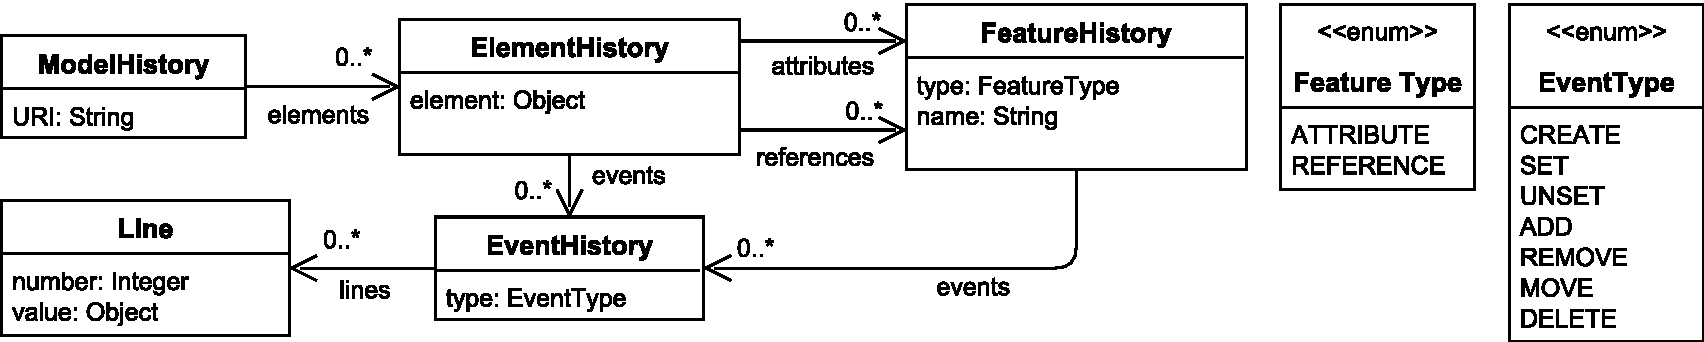
\includegraphics[width=\linewidth]{object_history}
    \caption{The class model defining Model History.}
    \label{fig:object_history}
\end{figure}
\end{frame}

\begin{frame}
\section{Optimising Set and Unset Events (1)}
\frametitle{Optimising Set and Unset Events (1)}
\begin{itemize}
    \item Track all line numbers of $SET$ and $UNSET$ events applied to an element' feature.
    \item If $SET$ event is the last event then it cancels all preceding $SET$ and $UNSET$ events.
    \item If $UNSET$ event is the last event then all $SET$ and $UNSET$ events are cancelled.
    \item All line numbers of the cancelled events are put into the ignore list. 
    \item All events referred by the line numbers in the ignore list are not replayed when loading a CBP.
\end{itemize}
\end{frame}

\begin{frame}[fragile]
\section{Optimising Set and Unset Events (2)}
\frametitle{Optimising Set and Unset Events (2)}
\begin{columns}
\begin{column}[t]{0.49\linewidth}
\begin{lstlisting}[style=eol,caption={A CBP representation of attribute \emph{name} assignments ended with SET.},label=lst:set_unset_example_1]
create n1 type Node
set n1.name to "A"
unset n1.name
set n1.name to "B"
\end{lstlisting}

\textbf{\footnotesize Model History}:\\
$name$.$set$.$lines$ = $\{\boldsymbol{2},4\}$\\
$name$.$unset$.$lines$ = $\{\boldsymbol{3}\}$\\
$ignoreList$ = $\{\boldsymbol{2}, \boldsymbol{3}\}$

\end{column}
\begin{column}[t]{0.49\linewidth}
\begin{lstlisting}[style=eol,caption={A CBP representation of attribute \emph{name} assignments ended with UNSET.},label=lst:set_unset_example_2]
create n1 type Node
set n1.name to "A"
set n1.name to "B"
unset n1.name
\end{lstlisting}

\textbf{\footnotesize Model History}:\\
$name$.$set$.$lines$ = $\{\boldsymbol{2},\boldsymbol{3}\}$\\ 
$name$.$unset$.$lines$ = $\{\boldsymbol{4}\}$\\
$ignoreList$ = $\{\boldsymbol{2}, \boldsymbol{3}, \boldsymbol{4}\}$

\end{column}
\end{columns}
\end{frame}


\begin{frame}
\section{Optimising Add, Remove, and Move Events (1)}
\frametitle{Optimising Add, Remove, and Move Events (1)}
\begin{itemize}
    \item Track all $ADD$, $REMOVE$, and $MOVE$ events applied to an element' multi-valued feature.
    \item If $ADD$ event is the last event, it cancels all preceding $ADD$ and $REMOVE$ events.
    \item If $REMOVE$ event is the last event, all $ADD$ and $REMOVE$ events are cancelled. 
    \item When a $MOVE$ event is applied, a flag \textbf{*isMoved} is set to \textbf{true} and the two rules are ignored since they can cause a \textbf{premature order} of the feature's values.
    \item If the feature is empty then \textbf{*isMoved} is set to \textbf{false} and all $ADD$, $REMOVE$, and $MOVE$ events are cancelled.
    \item All the line numbers of the cancelled events are put into the ignore list.
\end{itemize}
\end{frame}

\begin{frame}[fragile]
\section{Optimising Add, Remove, and Move Events (2)}
\frametitle{Optimising Add, Remove, and Move Events (2)}

\begin{columns}
\begin{column}[t]{0.5\linewidth}
\begin{lstlisting}[style=eol,caption={A CBP of add and remove operations.},label=lst:add_move_reference]
create p type Node
create n1 type Node
create n2 type Node
create n3 type Node
add n1 to p.children
add n2 to p.children
add n3 to p.children
remove n2 from p.children
   
\end{lstlisting}

\begin{footnotesize}
\textbf{Model History}:\\
$children$.$add$.$lines$ = \{\{5, $n1$\}, \{\textbf{6}, $n2$\} \{7, $n3$\}\}\\
$children$.$remove$.$lines$ = \{\{\textbf{8}, $n1$\}\}\\
$ignoreList$ = \{\textbf{6}, \textbf{8}\}
\end{footnotesize}

\end{column}
\begin{column}[t]{0.5\linewidth}
\begin{lstlisting}[style=eol,caption={A CBP representation of add, move, and remove operations.},label=lst:add_remove_move_reference]
create p type Node         
create n1 type Node        
create n2 type Node        
create n3 type Node        
add n1 to p.children     
add n2 to p.children     
add n3 to p.children     
move 0 to 1 in p.children
remove n2 from p.children
\end{lstlisting}

\begin{footnotesize}
\textbf{Model History}:\\
$children$.$add$.$lines$ = \{\{5, $n1$\}, \{\textbf{6}, $n2$\} \{7, $n3$\}\}\\
$children$.$move$.$lines$ = \{\{8, $n1$\}\}\\
$children$.$remove$.$lines$ = \{\{\textbf{9}, $n2$\}\}\\
$ignoreList$ = \{\textbf{6}, \textbf{9}\}\\
$p$.$children$ = [$n1$, $n3$]
\end{footnotesize}

\end{column}
\end{columns}

\end{frame}


\begin{frame}[fragile]
\section{Optimising Add, Remove, and Move Events (3)}
\frametitle{Optimising Add, Remove, and Move Events (3)}

\begin{columns}
\begin{column}[t]{0.52\linewidth}
\begin{lstlisting}[style=eol,caption={A replay of the CBP in Listing 6 after naive optimisation (without $*isMoved$ flag).},label=lst:naive_add_remove_move_reference]
create p type Node       *(1) 
create n1 type Node       (2)
create n2 type Node       (3)
create n3 type Node       (4)
add n1 to p.children      (5)
add n3 to p.children      (7) 
move 0 to 1 in p.children (8)
\end{lstlisting}

\begin{footnotesize}
\textbf{Model History}:\\
No $*isMoved$ flag\\
*previous line numbers\\
Previous $ignoreList$ = \{6, 9\}\\
$p$.$children$ = [$n3$, $n1$]
\end{footnotesize}

\end{column}
\begin{column}[t]{0.48\linewidth}
\begin{lstlisting}[style=eol,caption={A replay of the CBP in Listing 6 after optimisation with $*isMoved$ flag.},label=lst:add_remove_move_reference_with_flag]
create p type Node         
create n1 type Node        
create n2 type Node        
create n3 type Node        
add n1 to p.children     
add n2 to p.children     
add n3 to p.children     
move 0 to 1 in p.children
remove n2 from p.children
\end{lstlisting}

\begin{footnotesize}
\textbf{Model History}:\\
With $*isMoved$ flag = true\\
Previous $ignoreList$ = \{ \}\\
$p$.$children$ = [$n1$, $n3$]
\end{footnotesize}

\end{column}
\end{columns}

\end{frame}



\begin{frame}[fragile]
\section{Optimising Create and Delete Events (1)}
\frametitle{Optimising Create and Delete Events (1)}
\begin{itemize}
    \item Track all line numbers of all events ($CREATE$, $DELETE$, $ADD$, $REMOVE$, $MOVE$, $SET$, $UNSET$) applied to an element. 
    \item When an element is deleted, collect all the line numbers of the events into the ignore list.
    \item The line numbers in the ignore list indicate the events that are not replayed when loading a CBP.
\end{itemize}
\end{frame}

\begin{frame}[fragile]
\section{Optimising Create and Delete Events (2)}
\frametitle{Optimising Create and Delete Events (2)}

\begin{columns}
\begin{column}[t]{0.5\linewidth}
\begin{lstlisting}[style=eol,caption={A tree model persisted in change-based.},label=lst:cbpmodel]
create n1 type Node
set n1.name to "A"  
create n2 type Node
set n2.name to "B"  
create n3 type Node
set n3.name to "C"  
add n2 to n1.children   
add n3 to n1.children
remove n3 from n1.children   
delete n3
\end{lstlisting}

\begin{footnotesize}
\textbf{Model History}:\\
$n3$.$create$.$lines$ = \{\textbf{5}\}\\ 
$n3$.$name$.$set$.$lines$ = \{\textbf{6}\}\\
$n1$.$children$.$add$.$lines$ = \{\{7, $n2$\}, \{\textbf{8}, $n3$\}\}\\
$n1$.$children$.$remove$.$lines$ = \{\{\textbf{9}, $n3$\}\}\\
$n3$.$delete$.$lines$ = \{\textbf{10}\}\\
$ignoreList$ = \{\textbf{5}, \textbf{6}, \textbf{8}, \textbf{9}, \textbf{10}\}
\end{footnotesize}

\end{column}

\begin{column}[t]{0.5\linewidth}
\begin{lstlisting}[style=eol,caption={A replay of the CBP in Listing 9 after optimisation.},label=lst:cbpmodel_optimised]
create n1 type Node  *(1)
set n1.name to "A"    (2)
create n2 type Node   (3)
set n2.name to "B"    (4)
add n2 to n1.children (7)
\end{lstlisting}
*previous line numbers\\
\end{column}
\end{columns}

\end{frame}



\begin{frame}[fragile]
\section{Evaluation}
\frametitle{Evaluation}
\begin{itemize}
    \item Synthetic CBP models were derived from:
    \begin{itemize}
        \item UML2 models of the Epsilon and BPMN2 repositories.
        \item Modisco XML models of the Wikipedia's United States article.
    \end{itemize}
\end{itemize}
\hfill
\begin{scriptsize}
\begin{table} [ht]
\centering
\caption{Description of change-based models generated for evaluation.}
\label{table:data_description}
\begin{tabular}{>{\centering\arraybackslash}p{1.1cm}>{\centering\arraybackslash}p{1.1cm}>{\centering\arraybackslash}p{1.1cm}>{\centering\arraybackslash}p{1.1cm}
>{\centering\arraybackslash}p{1.2cm}>{\centering\arraybackslash}p{1.4cm}}
\hline 
\textbf{Model} & \textbf{Total Events} & \textbf{Ignored Events} & \textbf{Ignore \%} & \textbf{Elements} & \textbf{Processed Versions} \\
\hline
BPMN2 & \multicolumn{1}{r}{1.2 million} & \multicolumn{1}{r}{1.1 million} & \multicolumn{1}{r}{92\%} & \multicolumn{1}{r}{62,062} & \multicolumn{1}{r}{192} \\
%        BPMN2 & \multicolumn{1}{r|}{1,238,752} & \multicolumn{1}{r|}{1,078,058 (87.0\%)} & \multicolumn{1}{r|}{62,062} & \multicolumn{1}{r|}{192} & \multicolumn{1}{r|}{192 (100.0\%)} \\
Epsilon & \multicolumn{1}{r}{2.6 million} & \multicolumn{1}{r}{1.8 million} & \multicolumn{1}{r}{69\%} & \multicolumn{1}{r}{79,459} & \multicolumn{1}{r}{727} \\
%        Epsilon & \multicolumn{1}{r|}{2,593,044} & \multicolumn{1}{r|}{1,775,895 (68.5\%)} & \multicolumn{1}{r|}{79,459} & \multicolumn{1}{r|}{3,037} & \multicolumn{1}{r|}{727 (23.9\%)} \\
Wikipedia & \multicolumn{1}{r}{11.5 million} & \multicolumn{1}{r}{7.8 million} & \multicolumn{1}{r}{68\%} & \multicolumn{1}{r}{12,144} & \multicolumn{1}{r}{3,100} \\
%        Wikipedia & \multicolumn{1}{r|}{11,488,143} & \multicolumn{1}{r|}{7,765,000  (67.6\%)} & \multicolumn{1}{r|}{12,144} & \multicolumn{1}{r|}{37,996} & \multicolumn{1}{r|}{3,100 (8.2\%)} \\
\hline 
\end{tabular}
\end{table}
\end{scriptsize}
\end{frame}

\begin{frame}[fragile]
\section{Model Loading: Time}
\frametitle{Model Loading: Time}
Results for loading a model in original CBP (CBP), optimised CBP (OCBP), and for loading a state-based (XMI) representation.
\begin{figure}[ht]
    \begin{subfigure}{0.325\textwidth}
        \centering
        \includegraphics[width=\linewidth]{load_time_bpmn2}
        \caption{BPMN2}
        \label{fig:load_time_bpmn2}
    \end{subfigure}
    \hfill
    \begin{subfigure}{0.325\textwidth}
        \centering
        \includegraphics[width=\linewidth]{load_time_epsilon}
        \caption{Epsilon}
        \label{fig:load_time_epsilon}
    \end{subfigure}
    \hfill
    \begin{subfigure}{0.325\textwidth}
        \centering
        \includegraphics[width=\linewidth]{load_time_wikipedia}
        \caption{Wikipedia}
        \label{fig:load_time_wikipedia}
    \end{subfigure}
    \label{fig:loadtime}
\end{figure}
\begin{itemize}
    \item  BPMN2: Optimised CBP is 48.02\% faster than original CBP
    \item  Epsilon: Optimised CBP is 50.12\% faster than original CBP
    \item  Wikipedia: Optimised CBP is 23.63\% faster than original CBP
\end{itemize}

\end{frame}

\begin{frame}[fragile]
\section{Model Loading: Memory Footprint}
\frametitle{Model Loading: Memory Footprint}
A comparison on memory footprint after loading a model between original CBP (CBP), optimised CBP (OCBP), and XMI.
\begin{figure}[ht]
    \begin{subfigure}{0.325\textwidth}
        \centering
        \includegraphics[width=\linewidth]{load_memory_bpmn2}
        \caption{BPMN2}
        \label{fig:load_memory_bpmn2}
    \end{subfigure}
    \hfill
    \begin{subfigure}{0.325\textwidth}
        \centering
        \includegraphics[width=\linewidth]{load_memory_epsilon}
        \caption{Epsilon}
        \label{fig:load_memory_epsilon}
    \end{subfigure}
    \hfill
    \begin{subfigure}{0.325\textwidth}
        \centering
        \includegraphics[width=\linewidth]{load_memory_wikipedia}
        \caption{Wikipedia}
        \label{fig:load_memory_wikipedia}
    \end{subfigure}
    \label{fig:loadmemory}
\end{figure}
Optimised CBP uses significant memory overhead of the extra data structure when loading models.
\end{frame}

\begin{frame}[fragile]
\section{Model Saving: Time}
\frametitle{Model Saving: Time}
A comparison on time required for persisting an event between original CBP (CBP), optimised CBP (OCBP), and XMI.
\begin{figure}[t]
    \begin{subfigure}{0.325\textwidth}
        \centering
        \includegraphics[width=\linewidth]{save_time_bpmn2}
        \caption{BPMN2}
        \label{fig:save_time_bpmn2}
    \end{subfigure}
    \hfill
    \begin{subfigure}{0.325\textwidth}
        \centering
        \includegraphics[width=\linewidth]{save_time_epsilon}
        \caption{Epsilon}
        \label{fig:save_time_epsilon}
    \end{subfigure}
    \hfill
    \begin{subfigure}{0.325\textwidth}
        \centering
        \includegraphics[width=\linewidth]{save_time_wikipedia}
        \caption{Wikipedia}
        \label{fig:save_time_wikipedia}
    \end{subfigure}
    \label{fig:savetime}
\end{figure}
Optimised CBP and original CBP are faster in saving changes compared to XMI.
\end{frame}

\begin{frame}[fragile]
\section{Model Saving: Memory Footprint}
\frametitle{Model Saving: Memory Footprint}
A comparison on memory footprint after persisting an event between CBP, optimised CBP, and XMI.
\begin{figure}
    \begin{subfigure}{0.325\textwidth}
        \centering
        \includegraphics[width=\linewidth]{save_memory_bpmn2}
        \caption{BPMN2}
        \label{fig:save_memory_bpmn2}
    \end{subfigure}
    \hfill
    \begin{subfigure}{0.325\textwidth}
        \centering
        \includegraphics[width=\linewidth]{save_memory_epsilon}
        \caption{Epsilon}
        \label{fig:save_memory_epsilon}
    \end{subfigure}
    \hfill
    \begin{subfigure}{0.325\textwidth}
        \centering
        \includegraphics[width=\linewidth]{save_memory_wikipedia}
        \caption{Wikipedia}
        \label{fig:save_memory_wikipedia}
    \end{subfigure}
    \label{fig:savememory}
\end{figure}
Optimised CBP and original CBP produce less memory footprint compared to XMI.
\end{frame}

\begin{frame}[fragile]
\section{Conclusions and Future Work}
\frametitle{Conclusions and Future Work}
\begin{itemize}
    \item Conclusions
    \begin{itemize}
        \item We proposes an efficient algorithm and supporting data structures for loading change-based models.
        \item Our results show considerable savings in terms of loading time with a negligible impact on saving time, but at the cost of a higher memory footprint.
    \end{itemize}
    \item Future Work
    \begin{itemize}
        \item Evaluate CBP against state-based persistence on real complex models.
        \item Investigate the impact of change-based model
        persistence on the performance of change detection, model comparison and merging in the context of collaborative modelling.
        \item Explore a hybrid persistence representation that offers a combination of state-based and change-based
        persistence.
    \end{itemize}   
\end{itemize}
\end{frame}



\begin{frame}[fragile]
\section{Q \& A}
\frametitle{Q \& A}
\begin{itemize}
    \item \begin{LARGE}
        Q \& A
    \end{LARGE}
    \item GitHub: \url{https://github.com/epsilonlabs/emf-cbp}
\end{itemize}
\end{frame}



\begin{frame}
\section{The Object Diagram of The Model History}
\frametitle{The Object Diagram of The Model History}
\begin{figure}[ht]
    \centering
    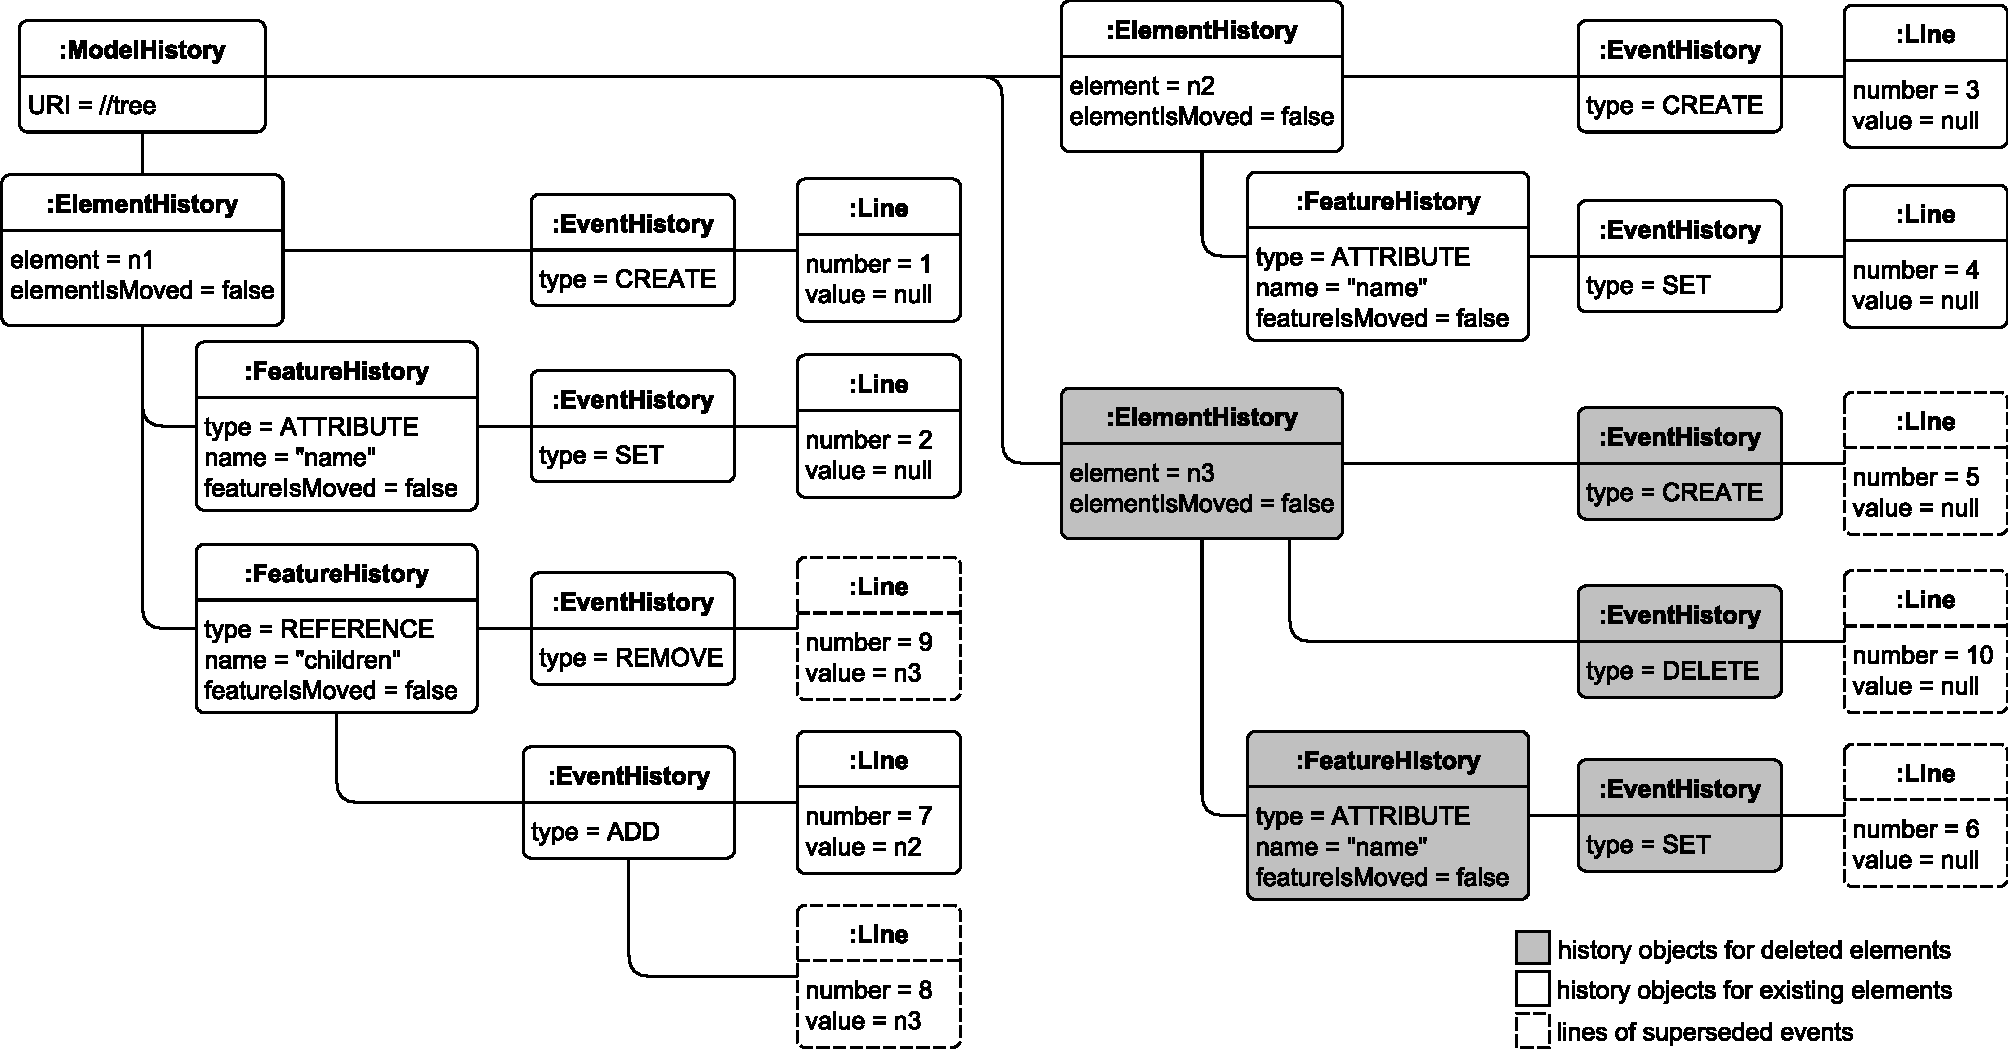
\includegraphics[width=\linewidth]{history_structure}
    \caption{The object diagram of the model history of the change-based tree model in Listing \ref{lst:cbpmodel}.}
    \label{fig:history_structure}
\end{figure}
\end{frame}

\begin{frame}
\section{Optimising Set and Unset Events (2)}
\frametitle{Optimising Set and Unset Events (2)}
\begin{algorithm}[H]
    \begin{small}
        \SetKwInOut{Input}{input}
        \SetKwInOut{Output}{output}
        \Input{a list of Integer $setEventNumbers$, a list of Integer $setEventNumbers$, a list of Integer $ignoreList$}
        \Output{a list of Integer $ignoreList$}
        \SetKwBlock{Beginn}{beginn}{ende}
        \Begin{
            $setLastLine$ $\leftarrow$ getLastLine($setEventNumbers$)\;
            $unsetLastLine$ $\leftarrow$ getLastLine($unsetEventNumbers$)\;
            \uIf{$setLastLine > unsetLastLine$}{
                $ignoreList \leftarrow (setEventNumbers \cup unsetEventNumbers) \setminus \{setLastLine\} $\;
            }
            \ElseIf{$setLastLine < unsetLastLine$}{
                $ignoreList \leftarrow (setEventNumbers \cup unsetEventNumbers)$\;
            }
            \Return{$ignoreList$}\;
        }
    \end{small}
    \caption{Algorithm to identify event numbers of superseded \emph{set} and \emph{unset} events}
    \label{alg:set_unset_optimisation}
\end{algorithm}
\end{frame}

\begin{frame}
\section{Optimising Add, Remove, and Move Events (3)}
\frametitle{Optimising Add, Remove, and Move Events (3)}
\begin{algorithm}[H]
    \begin{tiny}
        \SetKwInOut{Input}{input}
        \SetKwInOut{Output}{output}
        \SetKwProg{Struct}{struct}{}{end}
        \Struct{Line}{
            Integer $eventNumber$;
            Anytype $value$;
        }
        \Input{two lists of Line -- $addEventLines$ and $removeEventLines$, a variable of Anytype $operandValue$,  a list of Integer $ignoreList$, a variable of Boolean $featureIsMoved$} 
        \Output{a list of Integer $ignoreList$}
        \SetKwBlock{Beginn}{beginn}{ende}
        \Begin{
            \If{$featureIsMoved$ = false}{
                $filteredAddLines$ $\leftarrow$ filterByValue($addEventLines$, $operandValue$)\;
                $filteredRemoveLines$ $\leftarrow$ filterByValue($removeEventLines$, $operandValue$)\;
                $addLastLine$ $\leftarrow$ getLastLine($filteredAddLines$)\;
                $removeLastLine$ $\leftarrow$ getLastLine($filteredRemoveLines$)\;
                \uIf{$addLastLine > removeLastLine$}{
                    $ignoreList \leftarrow (filteredAddLines.eventNumbers \cup filteredRemoveLines.eventNumbers \setminus \{addLastLine\} $\;
                }
                \ElseIf{$addLastLine < removeLastLine$}{
                    $ignoreList \leftarrow (filteredAddLines.eventNumbers \cup filteredRemoveLines.eventNumbers$\;
                }
            }
            \Return{$ignoreList$}\;
        }
    \end{tiny}
    \caption{Algorithm to identify event numbers of superseded \emph{add}, \emph{remove}, and \emph{move} events.}
    \label{alg:add_remove_move_optimisation}
    
\end{algorithm}
\end{frame}

\begin{frame}[fragile]
\section{Optimising Create and Delete Events (2)}
\frametitle{Optimising Create and Delete Events (2)}
\begin{algorithm}[H]
    \begin{scriptsize}
        \SetKwInOut{Input}{input}
        \SetKwInOut{Output}{output}
        \Input{a variable of Object $deletedElement$, a list of Integer $ignoreList$}
        \Output{a list of Integer $ignoreList$}
        \Begin{
            $elementIsMoved$ $\leftarrow$ isElementMoved($deletedElement$)\;
            \If{$elementIsMoved$ = false}{
                $eventHistoryList$ $\leftarrow$ getAllEventHistories($deletedElement$)\; 
                \ForEach{$eventHistory$ in $EventHistoryList$}{
                    $lineList$ $\leftarrow$ getLines($eventHistory$)\;
                    Add all event numbers in $lineList$ into $ignoreList$\; 
                }
                $featureList$ $\leftarrow$ getAllAttributes($deletedElement$)\;
                \ForEach{$attribute$ in $featureList$}{
                    $eventHistoryList$ $\leftarrow$ getAllEventHistories($feature$)\;
                    \ForEach{$eventHistory$ in $EventHistoryList$}{
                        $lineList$ $\leftarrow$ getLines($eventHistory$)\;
                        Add all event numbers in $lineList$ into $ignoreList$\; 
                    }       
                }   
            }
            \Return{$ignoreList$}\;
        }
    \end{scriptsize}
    \caption{Algorithm to identify lines that are ignored after \emph{delete} events}
    \label{alg:create_delete_optimisation}
\end{algorithm}
\end{frame}




%\begin{frame}
%\section{References}
%\frametitle{References}
%\scriptsize
%\bibliographystyle{IEEEtran}
%\bibliography{references}
%\end{frame}
%
%\begin{frame}
%\cite{egyed2011automatically}
%\end{frame}
\end{document}
